\documentclass[UTF8]{article} 
\usepackage{graphicx}
\usepackage{subfigure}
\usepackage{amsmath}
\usepackage{makecell}
\usepackage[utf8]{inputenc}
\usepackage[space]{ctex} %中文包
\usepackage{listings} %放代码
\usepackage{xcolor} %代码着色宏包
\usepackage{CJK} %显示中文宏包
\usepackage{float}


\definecolor{mygreen}{rgb}{0,0.6,0}
\definecolor{mygray}{rgb}{0.5,0.5,0.5}
\definecolor{mymauve}{rgb}{0.58,0,0.82}
\lstset{
	backgroundcolor=\color{white}, 
	basicstyle = \footnotesize,       
	breakatwhitespace = false,        
	breaklines = true,                 
	captionpos = b,                    
	commentstyle = \color{mygreen}\bfseries,
	extendedchars = false,             
	frame =shadowbox, 
	framerule=0.5pt,
	keepspaces=true,
	keywordstyle=\color{blue}\bfseries, % keyword style
	language = Verilog,                     % the language of code
	otherkeywords={string}, 
	numbers=left, 
	numbersep=5pt,
	numberstyle=\tiny\color{mygray},
	rulecolor=\color{black},         
	showspaces=false,  
	showstringspaces=false, 
	showtabs=false,    
	stepnumber=1,         
	stringstyle=\color{mymauve},        % string literal style
	tabsize=4,          
	title=\lstname                      
}


\title{中国科学技术大学计算机学院\\《数字电路实验》报告}
\author{}

\date{}

\begin{document}
	\maketitle
	\begin{figure}[H]
		\centering
		
\includegraphics[width=2.5in]{xiaohui.jpg}\vspace{0.5cm}\\
		\large{
			实验题目:FPGA 实验平台及 IP 核使用\\
			学生姓名:王章瀚\\
			学生学号:PB18111697\\
			完成日期:\today\\
		}\vspace{2cm}
		
		\large{计算机实验教学中心制\\2019年09月\\}
		\thispagestyle{empty}
		\clearpage  % 清除当页页码
	\end{figure}


	\section{实验目的}
	学会查看原理图\par
	理解 FPGA 开发各关键环节\par
	学会使用 IP 核(知识产权核)\par
	
	\section{实验环境}
	PC 一台\par
	Windows 或 Linux 操作系统\par
	Logisim\par
	Vivado 工具\par
	FPGA 实验平台(Nexys4 DDR)\par
	vlab.ustc.edu.cn\par
	
	\section{实验过程}
	\subsection{Nexys4 DDR 开发板简介}
	Nexys4 DDR 开发板采用 Xilinx 的 XC7A100TCSG324C-1 为核心芯片, 配备了开关、按键、 LED 灯、数码管等多种基本外设,还支持 USB、RJ45、 VGA 等多种通用接口,以及五个用于扩展的 PMOD 接口,此外还放置了一颗 128MB 的 DDR 内存颗粒。\par
	以下是一张外设表:\par
	\begin{figure}[H]
		\centering
		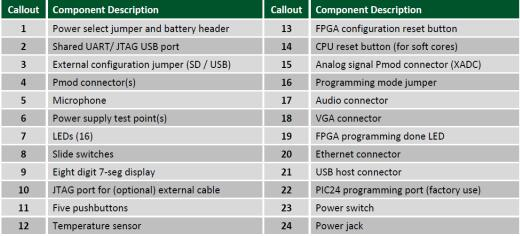
\includegraphics[width=1\linewidth]{s1.jpg}
		\label{s1}
	\end{figure}\par
	
	\subsection{开发板原理图介绍}
	Nexys4 DDR 开发板上通过丝印的形式标注了部分外设与 FPGA 管脚之间的连接方式。FPGA 的通用管脚既可以设置为输入和输出,而实际使用中,我们会根据通用管脚与外部电路的连接关系,固定的用来做输入或输入。了解开发板结构、连接关系以及其它技术细节的最有效的途径是查看说明文档和电路原理图。 下图给出了Nexys4DDR开发板FPGA与各种基本外设的连接关系:\par
	\begin{figure}[H]
		\centering
		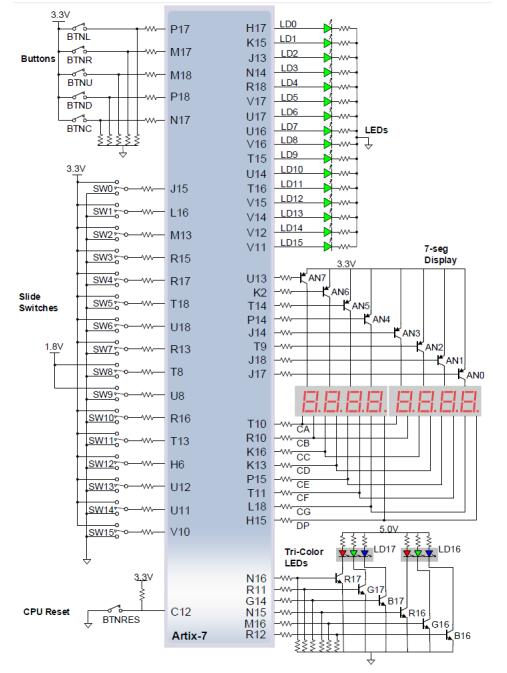
\includegraphics[width=1\linewidth]{s2_1.jpg}
		\label{s2_1}
	\end{figure}\par
	其中拨动开关和单刀双掷开关原理基本相同;五个按键通过下拉电阻和FPGA的五个通用管脚连接;16个LED都是P极接FPGA管脚,N 极通过限流电阻接地。\par
	4种基本外设中,最为复杂的是数码管电路。开发板上用的是共阳极数码管。FPGA 管脚通过三极管放大电路控制数码管的位选择信号,每个管脚对应一个数码管,且数码管的段选择信号是共用的。\par
	图中还有两个三色 LED,根据连接图可以看出,对应的 FPGA 管脚高电平有效。\par
	此外,通过查阅原理图,我们不仅可以了解到 FPGA芯片与各种外设之间的连接关系,还能了解到一些更加细节的地方。\par
	讲义图中的 FPGA 芯片,按供电、配置、通用 IO 等功能分成了 6 个部分。\par
	举例来说,上一次实验的时钟信号被分配到了 E3 管脚。通过查看原理图可以发现该 FPGA 管脚是与一个时钟芯片相连接的。\par
	\begin{figure}[H]
		\centering
		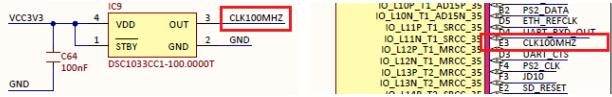
\includegraphics[width=1\linewidth]{s2_2.jpg}
		\label{s2_2}
	\end{figure}\par
	为避免每次建立工程时都要通过原理图查看管脚对应关系,我们可以使用官方提供的 Nexys4DDR 的 XDC 文件。\par
	
	\subsection{FPGAOL 平台介绍}
	该平台是包含20个节点的远程FPGA实验平台。每个节点包含一个 Nexys4DDR 开发板和一个树莓派单板,
	两者使用排线相连。树莓派对用户来说完全透明, 负责与服务器端进行通信,完成烧录 FPGA,对 FPGA 管脚信号进行实时采样等功能。\par
	该平台操作简单,界面直观,用户不需要购置硬件设备便可以完成 FPGA 开发流程的学习。\par
	
	\subsection{使用时钟管理单元 IP 核}
	在 FPGA 开发中,有很多常用功能的模块是不需要自己开发的,用户可以复用第三方开发好的模块,这种模块被称为 IP 核。\par
	例如,如果我们需要一个其它频率的时钟信号,例如 10MHz,应该怎么办呢?\par
	一般的做法是通过计数器产生一个低频的脉冲信号,然后再将该脉冲信号控制其他逻辑的控制信号。\par
	对讲义的代码进行仿真,能够得到如下波形图:\par
	\begin{figure}[H]
		\centering
		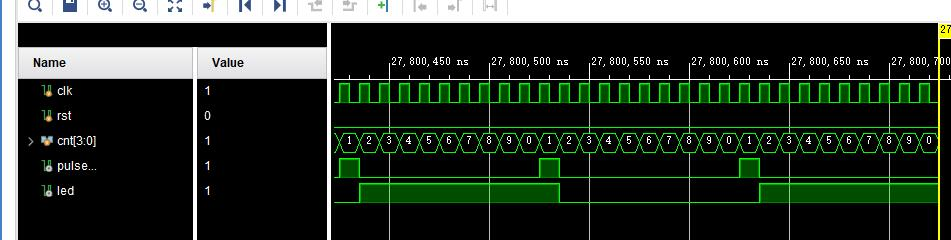
\includegraphics[width=1\linewidth]{s4_1.jpg}
		\label{s4_1}
	\end{figure}\par
	应记住:将分频信号直接作为时钟使用,会产生许多无谓的警告,也容易引起电路工作的不稳定。\par
	时钟信号是非常特殊的一种信号,它不应该出现在过程语句和连续赋值语句内部。时钟信号只应该出现在 always 语句的时序控制部分。\par
	如果设计中确实需要不同频率的时钟信号应该通过时钟管理单元 IP 核生成。\par 
	\begin{figure}[H]
		\begin{minipage}[H]{0.45\linewidth}
			\centering
			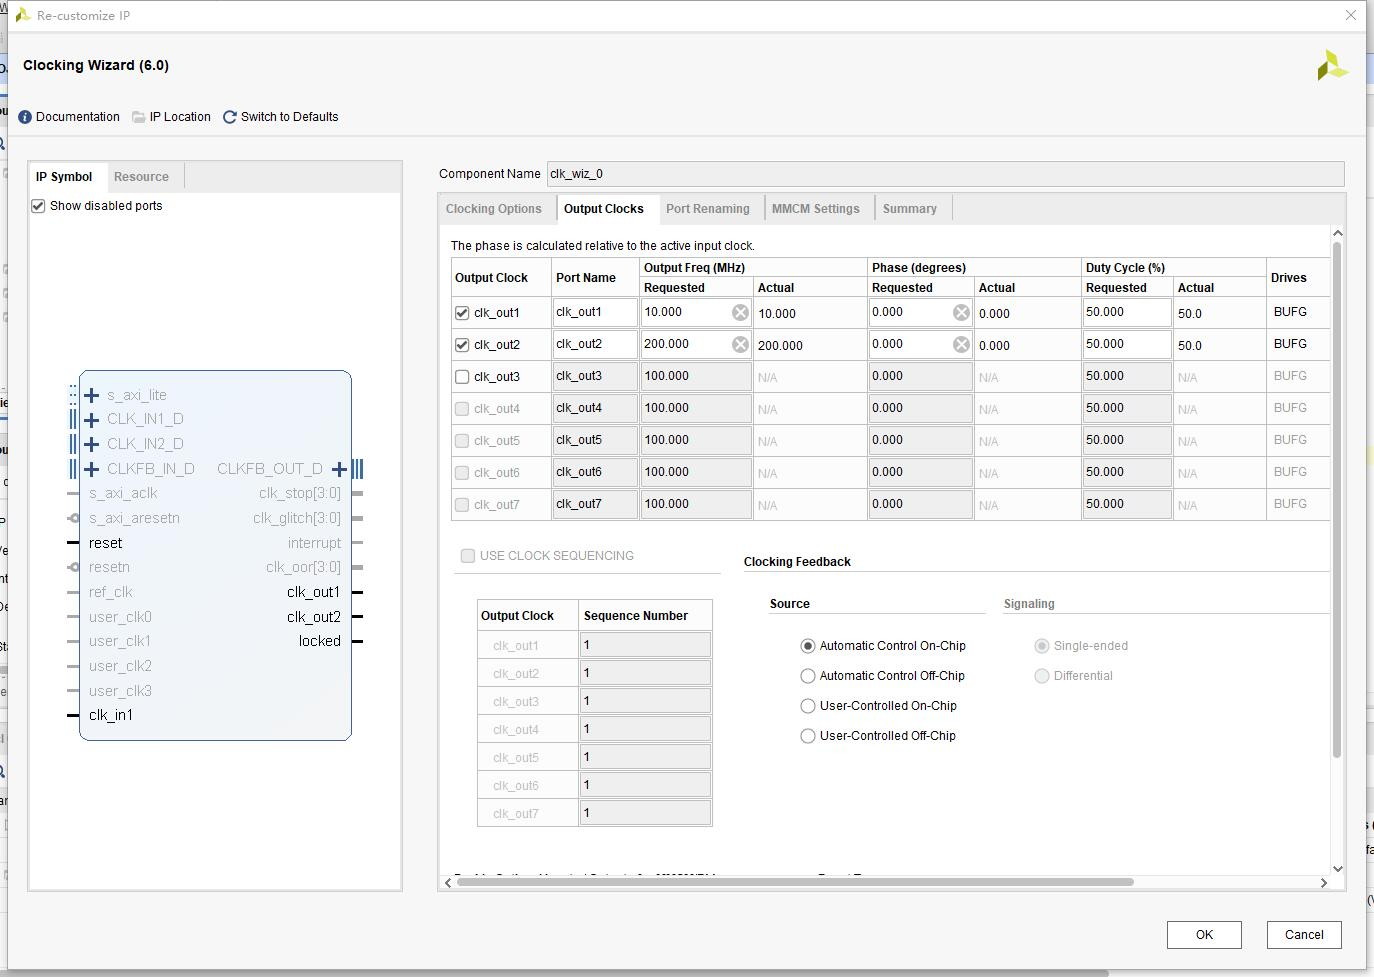
\includegraphics[scale=0.16]{s4_2.jpg}
			\label{s4_2}
		\end{minipage}
		\qquad
		\begin{minipage}[H]{0.45\linewidth}
			\centering
			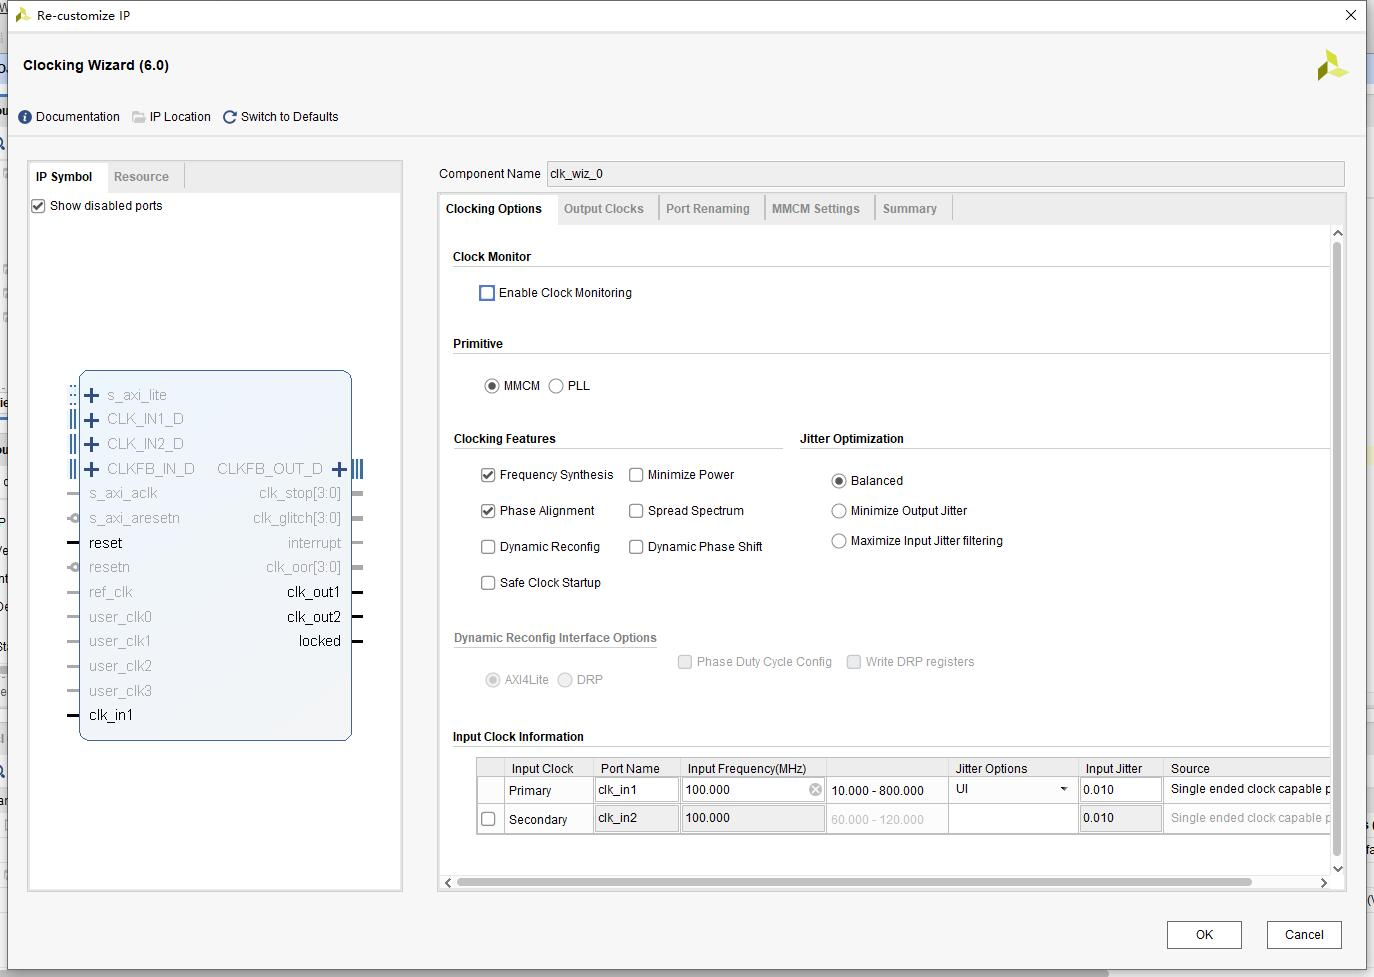
\includegraphics[scale=0.16]{s4_3.jpg}
			\label{s4_3}
		\end{minipage}
	\end{figure}
	分析讲义给出的代码,其是用于让LED灯显示计数的[27:24],并用以不同时钟频率。通过仿真和烧写 FPGA,可以发现两个时钟频率的明显差异。下图是波形图:\par
	\begin{figure}[H]
		\centering
		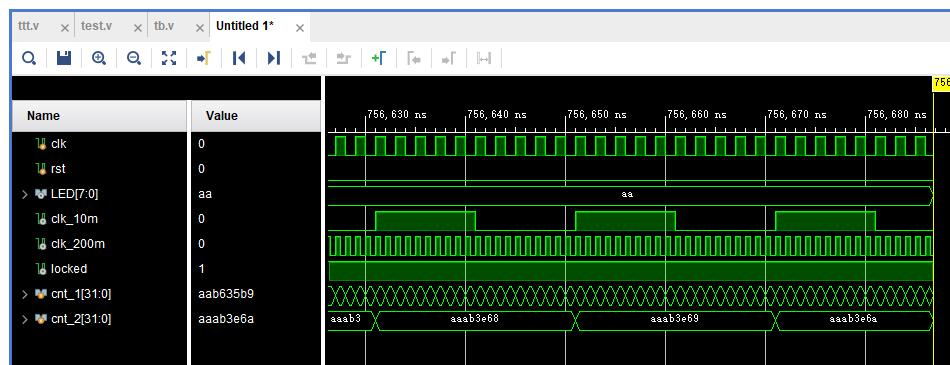
\includegraphics[scale=0.5]{s4_4.jpg}
		\label{s4_4}
	\end{figure}
	如果电路中需要一个较低频率的时序,例如我们需要一个每秒钟加一的计数器,那我们就只能通过前面介绍的方法,用周期为 1 秒的脉冲信号来控制了。\par
	
	\subsection{使用片内存储单元}
	我们可以从 ROM 读取数据,但无法通过端口修改其内容,与此相对应的是 RAM(随机存储器),其内容可读可写。\par
	Logisim 中的 RAM 模型,包含地址(A) 、数据(D,输入输入复用) 、片选(sel) 、	时钟(clk,数据可在时钟上升沿写入) 、 输出使能(ld,为 1 时数据端口为输出,否则为输入) 、清空(clr) 等端口信号。 这种 RAM 包含一套读写端口,因此成为单端口 RAM。 \par
	\begin{figure}[H]
		\centering
		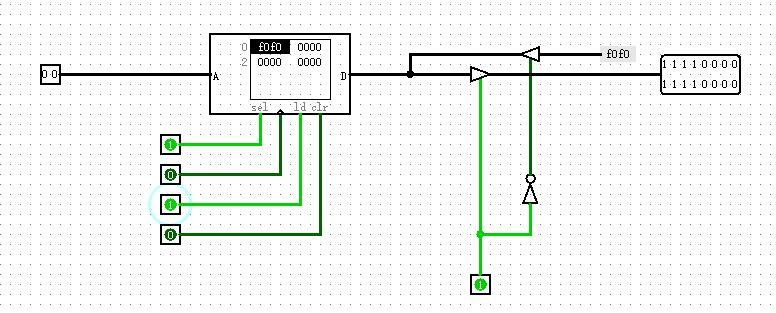
\includegraphics[width=1\linewidth]{s5.jpg}
		\label{s5}
	\end{figure}\par
	Vivao 中也提供了存储器相关的IP核。以下以Distributed Memory为例介绍。\par
	搭建后仿真结果如下:\par
	\begin{figure}[H]
		\centering
		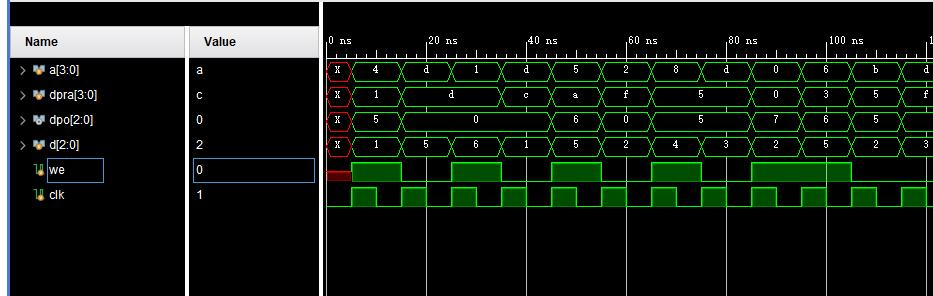
\includegraphics[width=1\linewidth]{s5_2.jpg}
		\label{s5_2}
	\end{figure}\par
	可以观察到下图结果:
	\begin{figure}[H]
		\centering
		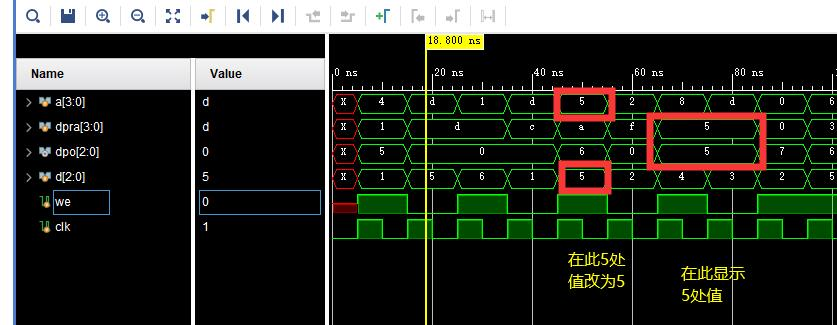
\includegraphics[width=1\linewidth]{s5_3.jpg}
		\label{s5_3}
	\end{figure}\par
	
	
	\section{实验练习}
	\subsection{题目1}
	对ROM的例化过程中,设置初始化值如下:\par
	\begin{figure}[H]
		\centering
		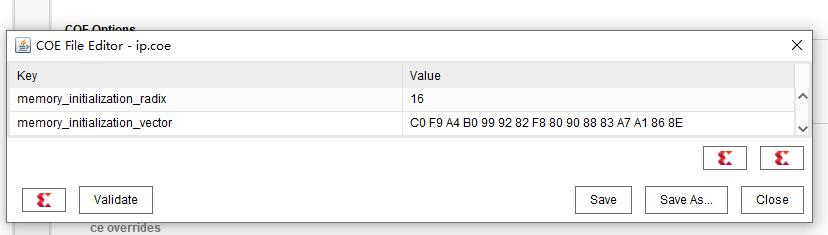
\includegraphics[width=1\linewidth]{e1_1.jpg}
		\label{e1_1}
	\end{figure}\par
	Verilog代码如下:
	\begin{lstlisting}[language=Verilog]
	module e1(
		input [3:0] SW,
		output [7:0] seg,
		output reg [7:0] AN
		);
	
	dist_mem_gen_0 dist_mem_gen_0(SW, seg);
	
	initial
	begin
		AN <= 8'b1111_1110;
	end
	
	endmodule
	\end{lstlisting}
	烧入FPGA中,由开关可以调整到所有数字,效果图如下(图中输入为1110,显示一个E):\par
	\begin{figure}[H]
		\centering
		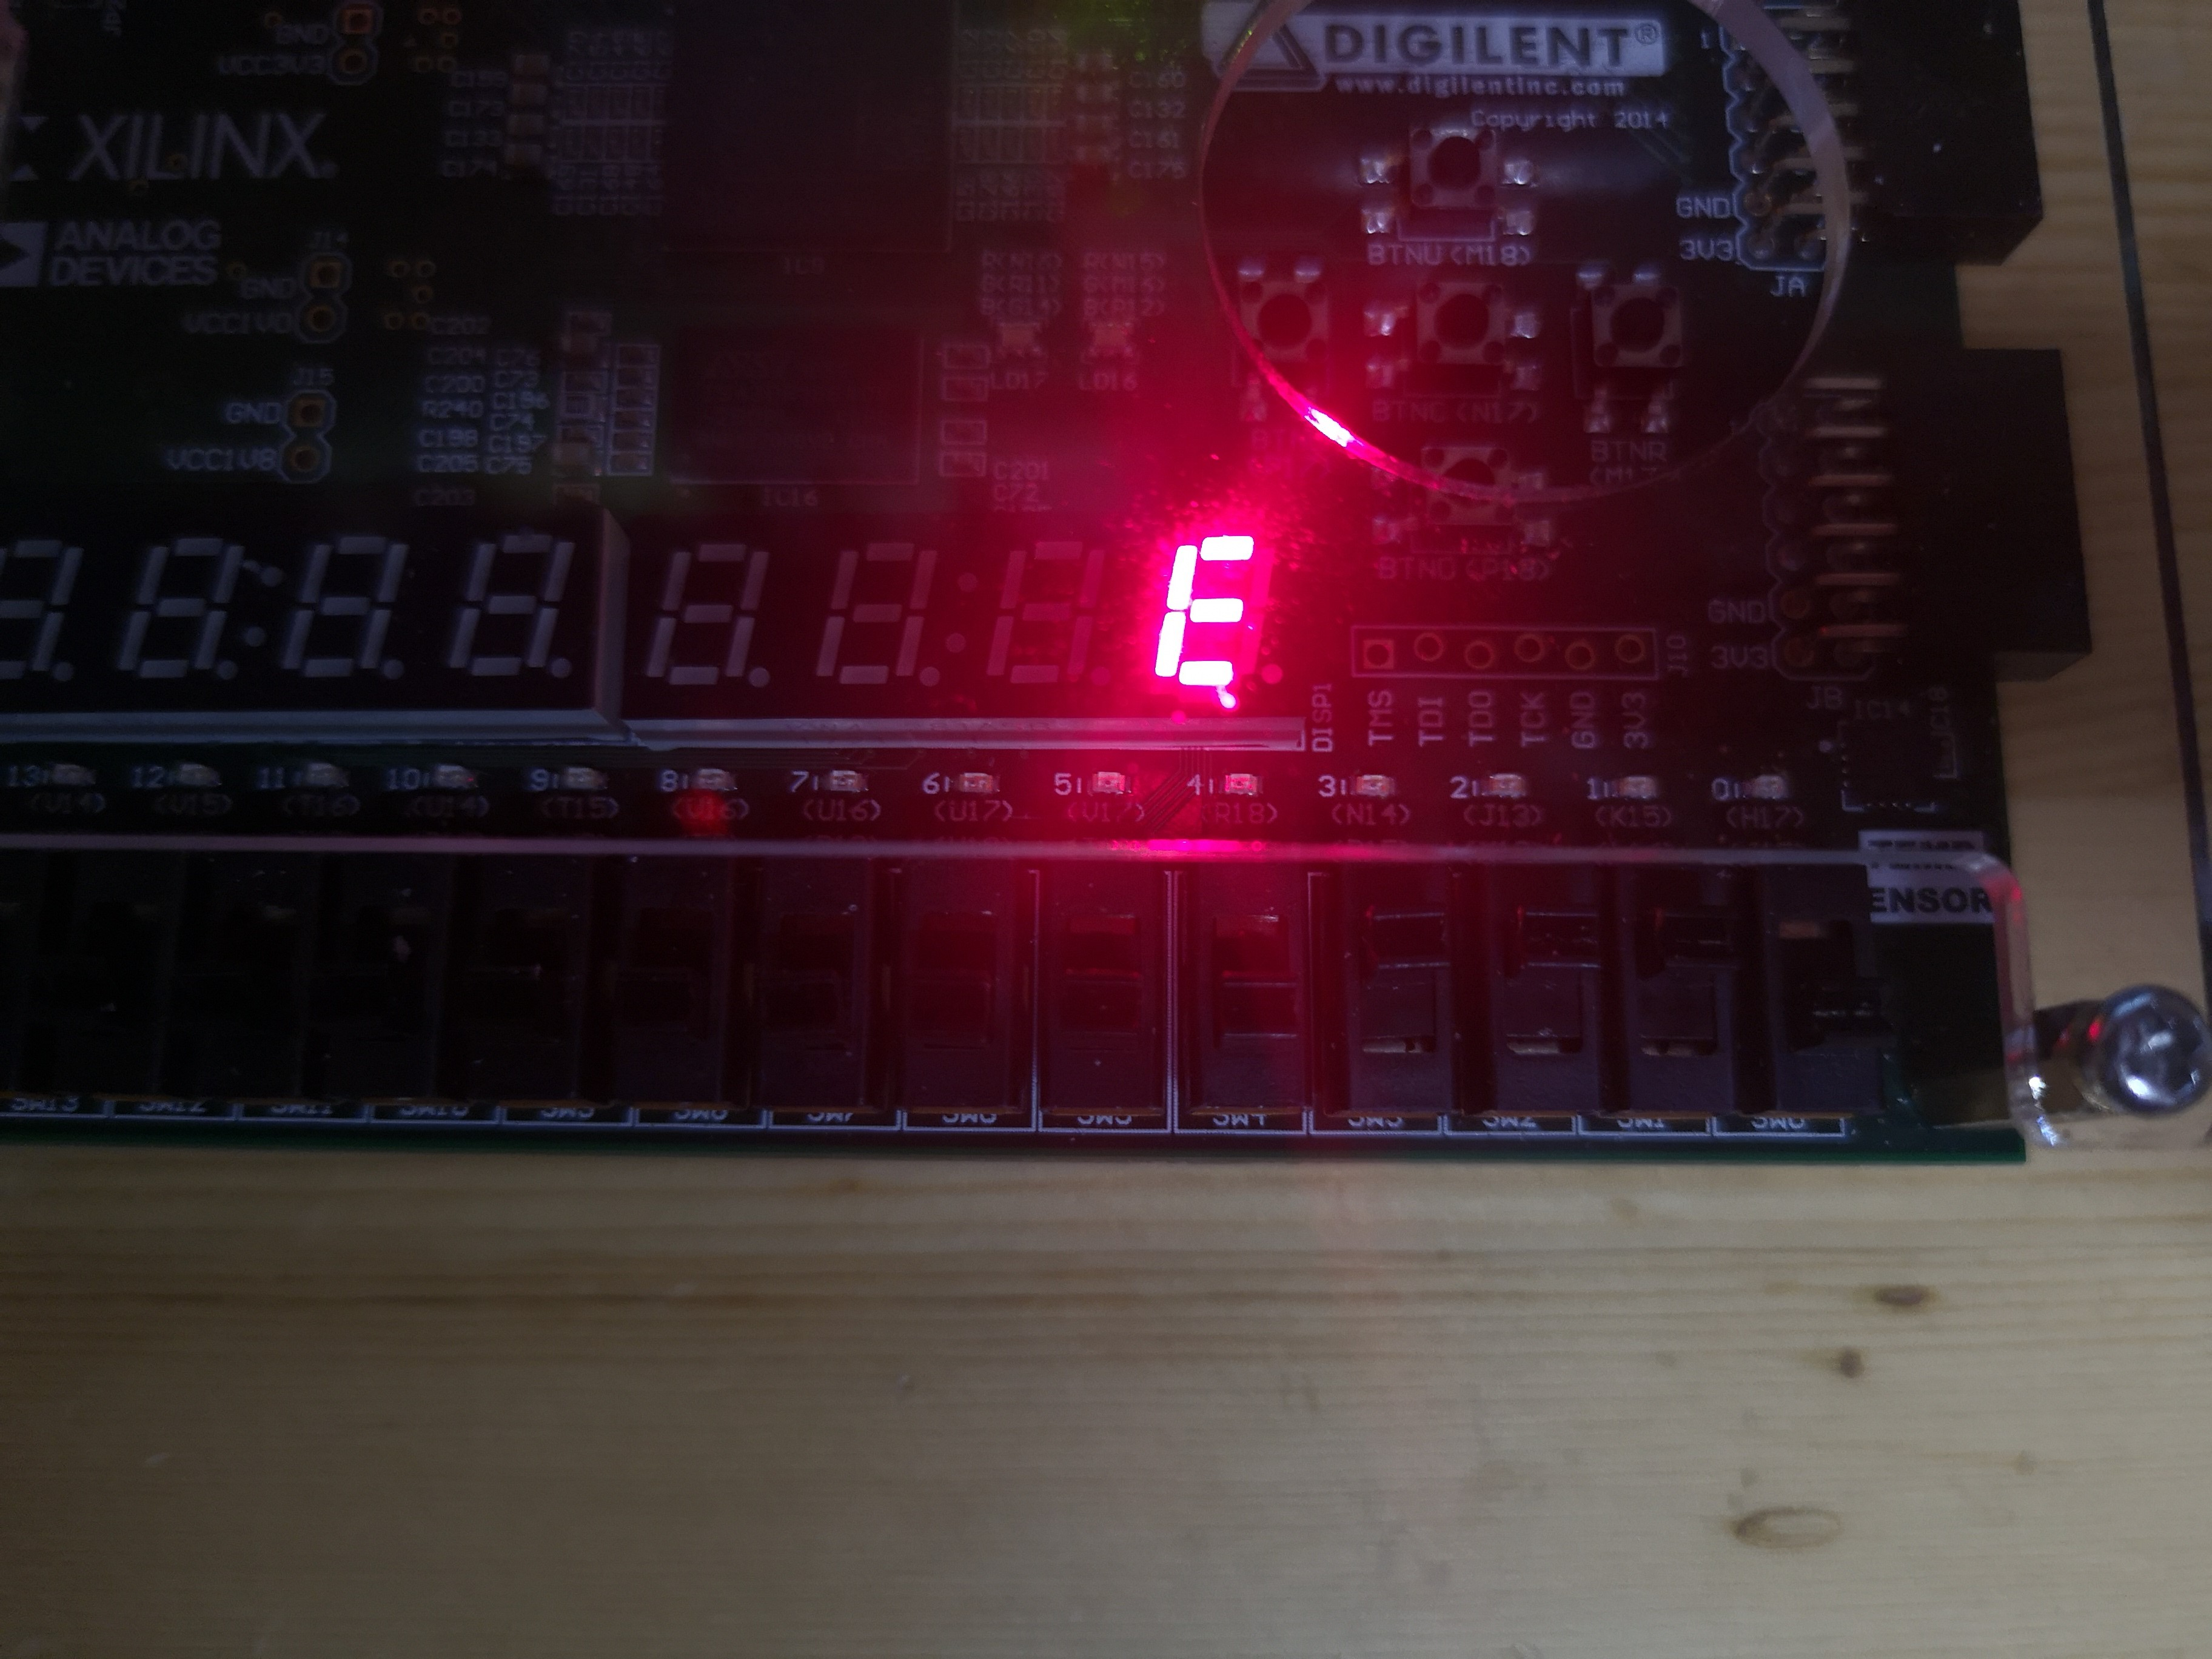
\includegraphics[width=1\linewidth]{e1_2.jpg}
		\label{e1_2}
	\end{figure}\par
	
	\subsection{题目2}
	对于多位数码管而言,时分复用的频率不必过高,因此采用计数器来产生一个低频信号。\par
	此外,为了显示数码管而生成的IP核与第一题的配置一致。\par
	使用代码如下:
	\begin{lstlisting}[language=Verilog]
	module e2(
		input [7:0] SW,
		input clk,
		output [7:0] seg,
		output reg [7:0] AN
		);
	
	integer counter;
	reg [3:0] data;
	
	dist_mem_gen_0 dist_mem_gen_0_1(data, seg);
	
	initial
	begin
		AN <= 8'b1111_1110;
		counter <= 0;
	end
	
	always @(posedge clk)
	begin
		if(counter == 100000)
			counter <= 0;
		else
			counter <= counter + 1;
	end
		
	always @(posedge clk)
	begin
		if(counter == 0)
		begin
		case(AN)
			8'b1111_1101 : begin AN <= 8'b1111_1110; data <= SW[3:0]; end
			default : begin AN <= 8'b1111_1101; data <= SW[7:4]; end
		endcase
	end
	end
	
	endmodule
	\end{lstlisting}
	经过烧写测试,有如下效果图:\par
	\begin{figure}[H]
		\centering
		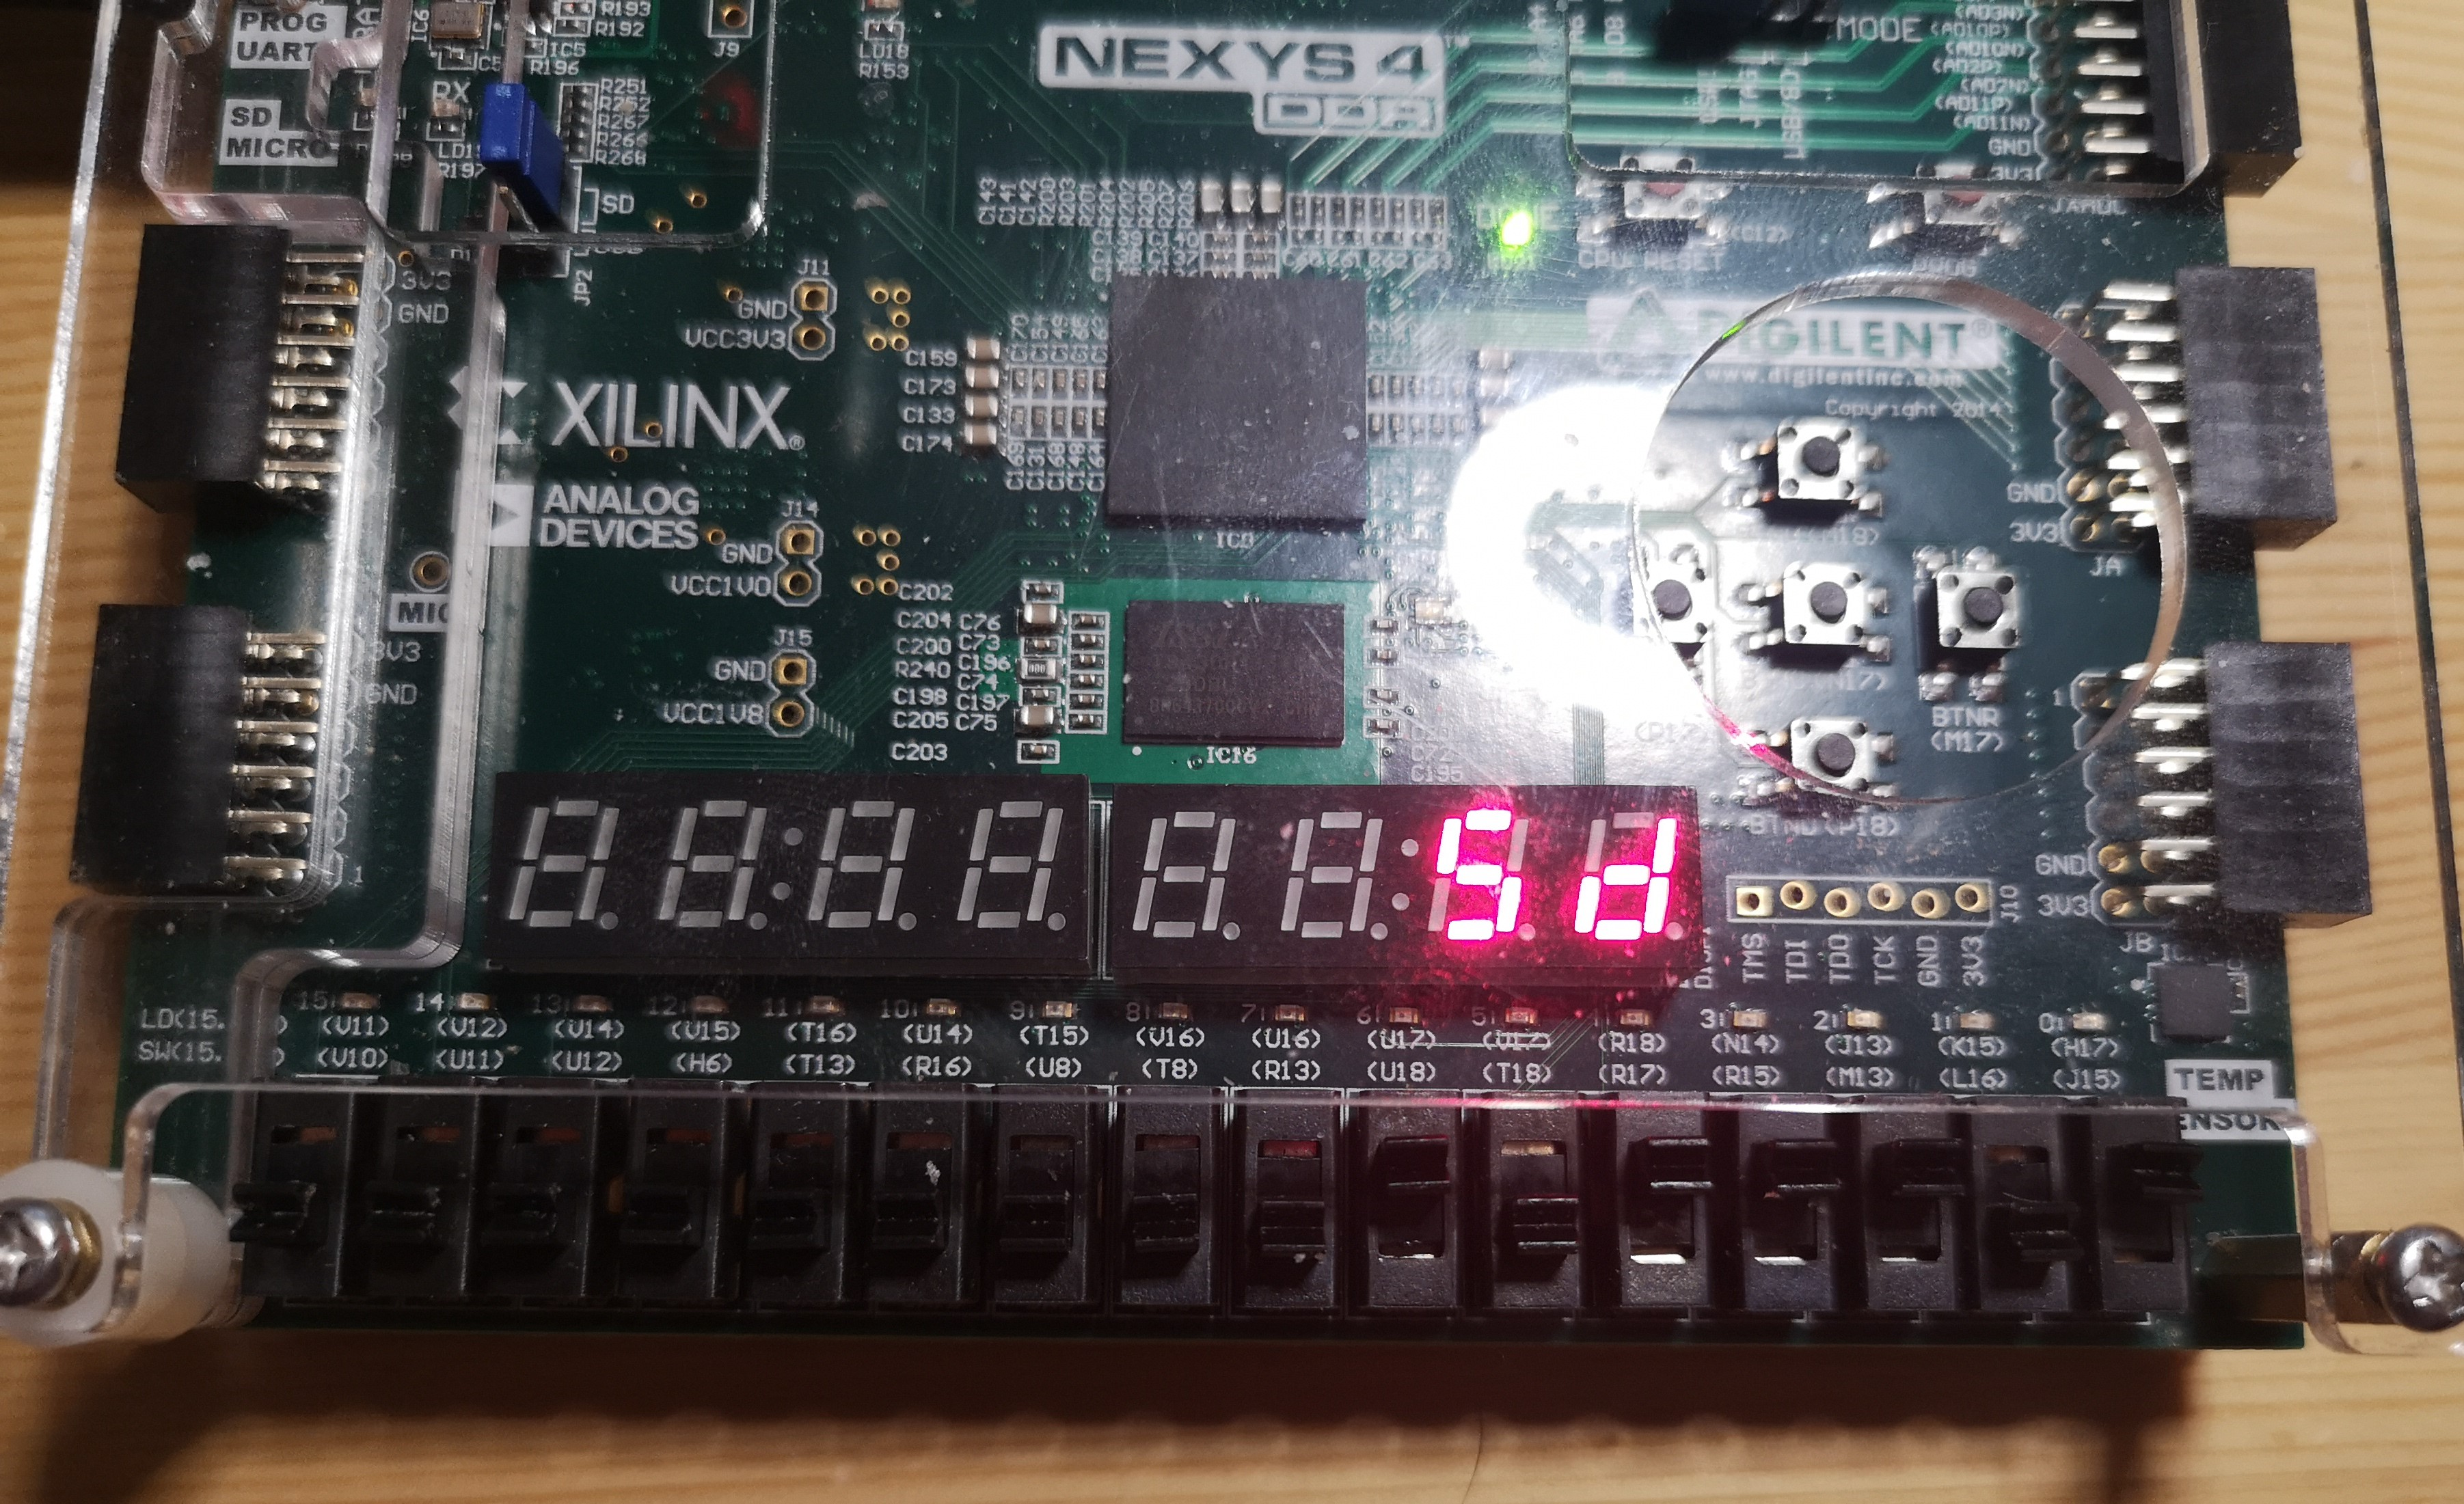
\includegraphics[width=1\linewidth]{e2_1.jpg}
		\label{e2_1}
	\end{figure}\par
	
	\subsection{题目3}
	首先声明本人对题目的理解:从1分23秒4开始倒计时,到0后重新开始。若按下复位,则复位到1分23秒4。\par
	原频率是100MHZ,不适合采用clocking wizard。因此直接采用周期脉冲方法,此时需要计数到10M。\par 
	此外,为了显示数码管而生成的IP核与第一题的配置一致。\par
	考虑到计时器需要复位功能,因此加入rst。\par
	代码如下:
	\begin{lstlisting}[language=Verilog]
	module e3(
		input clk, rst,
		output wire [7:0] seg,
		output reg [7:0] AN
		);
	
	integer cnt_target_1000HZ, cnt_target_10HZ;
	integer cnt_1000HZ, cnt_10HZ;
	reg [15:0] timer;
	reg [3:0] data;
	
	dist_mem_gen_0 dist_mem_gen_0(data, seg);
	
	initial
	begin
		cnt_10HZ <= 0;
		cnt_target_10HZ <= 10000000;
		cnt_10HZ <= 0;
		cnt_target_1000HZ <= 100000;
		AN <= 8'b1111_1110;
		data <= 0;
		timer = 16'h1234;
	end
	
	always @(posedge clk)
	begin
		cnt_1000HZ = cnt_1000HZ + 1;
		if(cnt_1000HZ == cnt_target_1000HZ)
		begin
			// 时分复用
			cnt_1000HZ = 0;
			case(AN)
				8'b1111_1011 : 
				begin 
					AN <= 8'b1111_0111; data <= timer[15:12]; 
				end
				8'b1111_1101 : 
				begin 
					AN <= 8'b1111_1011; data <= timer[11:8]; 
				end
				8'b1111_1110 : 
				begin 
					AN <= 8'b1111_1101; data <= timer[7:4]; 
				end
				8'b1111_0111 : 
				begin 
					AN <= 8'b1111_1110; data <= timer[3:0]; 
				end
				default : 
				begin
					AN <= 8'b1111_1110; data <= timer[3:0]; 
				end
			endcase
		end
	end
	
	always @(posedge clk or posedge rst)
	begin
		// 对timer进行10HZ的自加计时,其中包括特殊进位的处理
		if(rst == 1)
		begin   
			cnt_10HZ <= 0;
			timer <= 16'h1234;
		end
		else
		begin
			cnt_10HZ = cnt_10HZ + 1;
			if(cnt_10HZ == cnt_target_10HZ)
			begin
				cnt_10HZ = 0;
				if(timer == 16'h0000)
					timer = 16'h1234;
				else
				begin
					timer = timer - 1;
					if(timer[3:0] > 4'h9) // the bit needs borrow.
						timer[3:0] = 9;
					if(timer[7:4] > 4'h9) // the bit needs borrow.
						timer[7:4] = 9;
					if(timer[11:8] > 4'h5) // the bit needs borrow.
						timer[11:8] = 5; 
				end
			end
		end
	end
	
	endmodule
	\end{lstlisting}\par
	最后效果图如下:\par
	\begin{figure}[H]
		\centering
		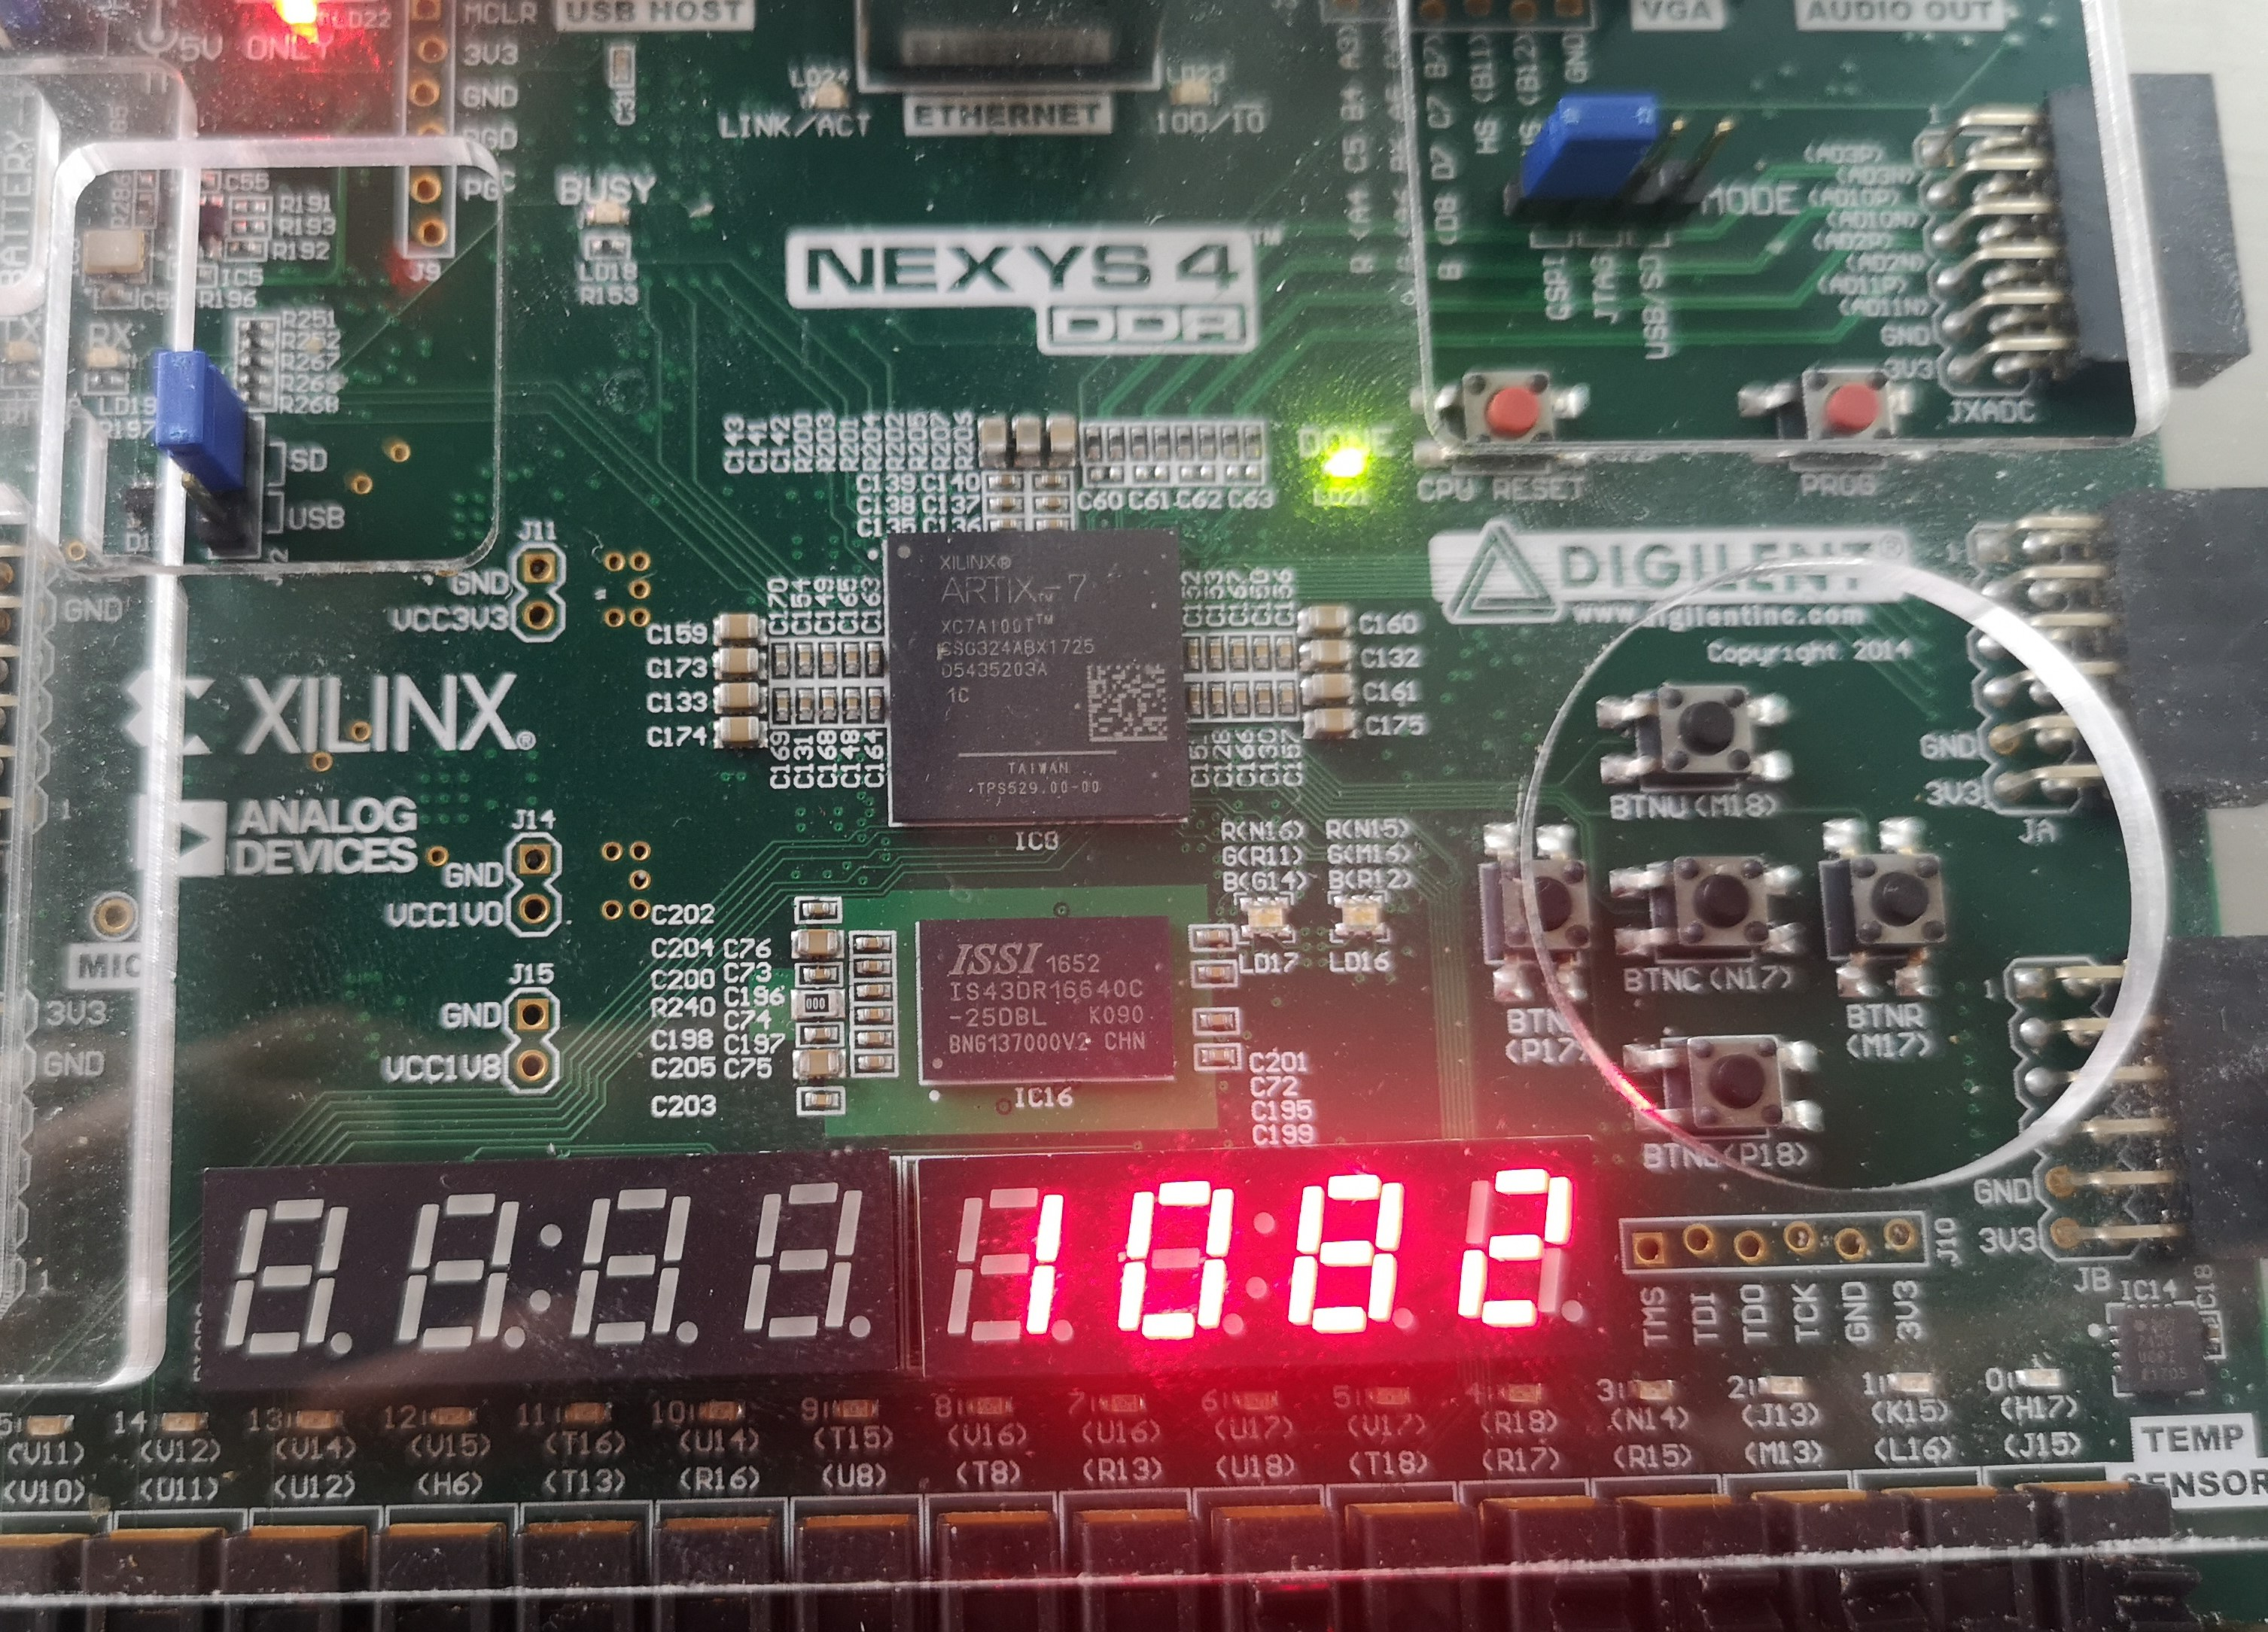
\includegraphics[width=1\linewidth]{e3_1.jpg}
		\label{e3_1}
	\end{figure}\par
	
	
	
	
	
	
	\section{总结与思考}	
	\subsection{本次实验的收获}
	在本次实验中,收获较大,学会了使用IP核,了解了七段数码管的控制。\par
	
	\subsection{评价本次实验的难易程度}
	本次实验内容难度适中。\par
	
	\subsection{评价本次实验的任务量}
	本次实验任务量较大。\par
	
	\subsection{为本次实验提供改进建议}
	建议对常用IP核给出一个索引表之类的东西,方便同学们使用与学习。\par
	
\end{document}
